\documentclass[border=1pt]{standalone}
\usepackage{tikz}
\usepackage{amsmath}
\usepackage{sansmath}
\usetikzlibrary{arrows.meta, positioning, calc, backgrounds, fit, decorations.pathreplacing, patterns}

% ===================== COLOUR PALETTE (shared with the other diagrams) =====================
\definecolor{cT}{HTML}{D85A30}    % tasmax
\definecolor{cH}{HTML}{1D9E75}    % rh (hurs)
\definecolor{cV}{HTML}{378ADD}    % pr
\definecolor{cInk}{HTML}{2B2B2B}
\definecolor{lightR}{HTML}{8FC1EE} % CMH-LP  <-- replace with the definition used in the paper
\definecolor{heavyR}{HTML}{1B5FA8} % CMH-HP  <-- replace with the definition used in the paper

\renewcommand{\familydefault}{\sfdefault}
\begin{document}
\sansmath

% ---------- heat map (illustrative climate field): x0, y0, side, n grids, colour, phase, detail ----------
\newcommand{\hmap}[7]{%
  \pgfmathsetmacro\cs{#3/#4}%
  \foreach \i in {1,...,#4}{\foreach \j in {1,...,#4}{%
    \pgfmathsetmacro\u{(\i-0.5)/#4}\pgfmathsetmacro\w{(\j-0.5)/#4}%
    \pgfmathsetmacro\val{max(12,min(100, 55+42*sin(230*\u+#6)*sin(200*\w+40+0.7*#6) + #7*sin(1700*\u+#6)*sin(1400*\w)))}%
    \fill[#5!\val!white] ({#1+(\i-1)*\cs},{#2+(\j-1)*\cs}) rectangle ++(\cs,\cs);}}%
  \draw[white, line width=0.25pt, step=\cs] (#1,#2) grid ++(#3,#3);
  \draw[cInk, line width=0.8pt] (#1,#2) rectangle ++(#3,#3);}

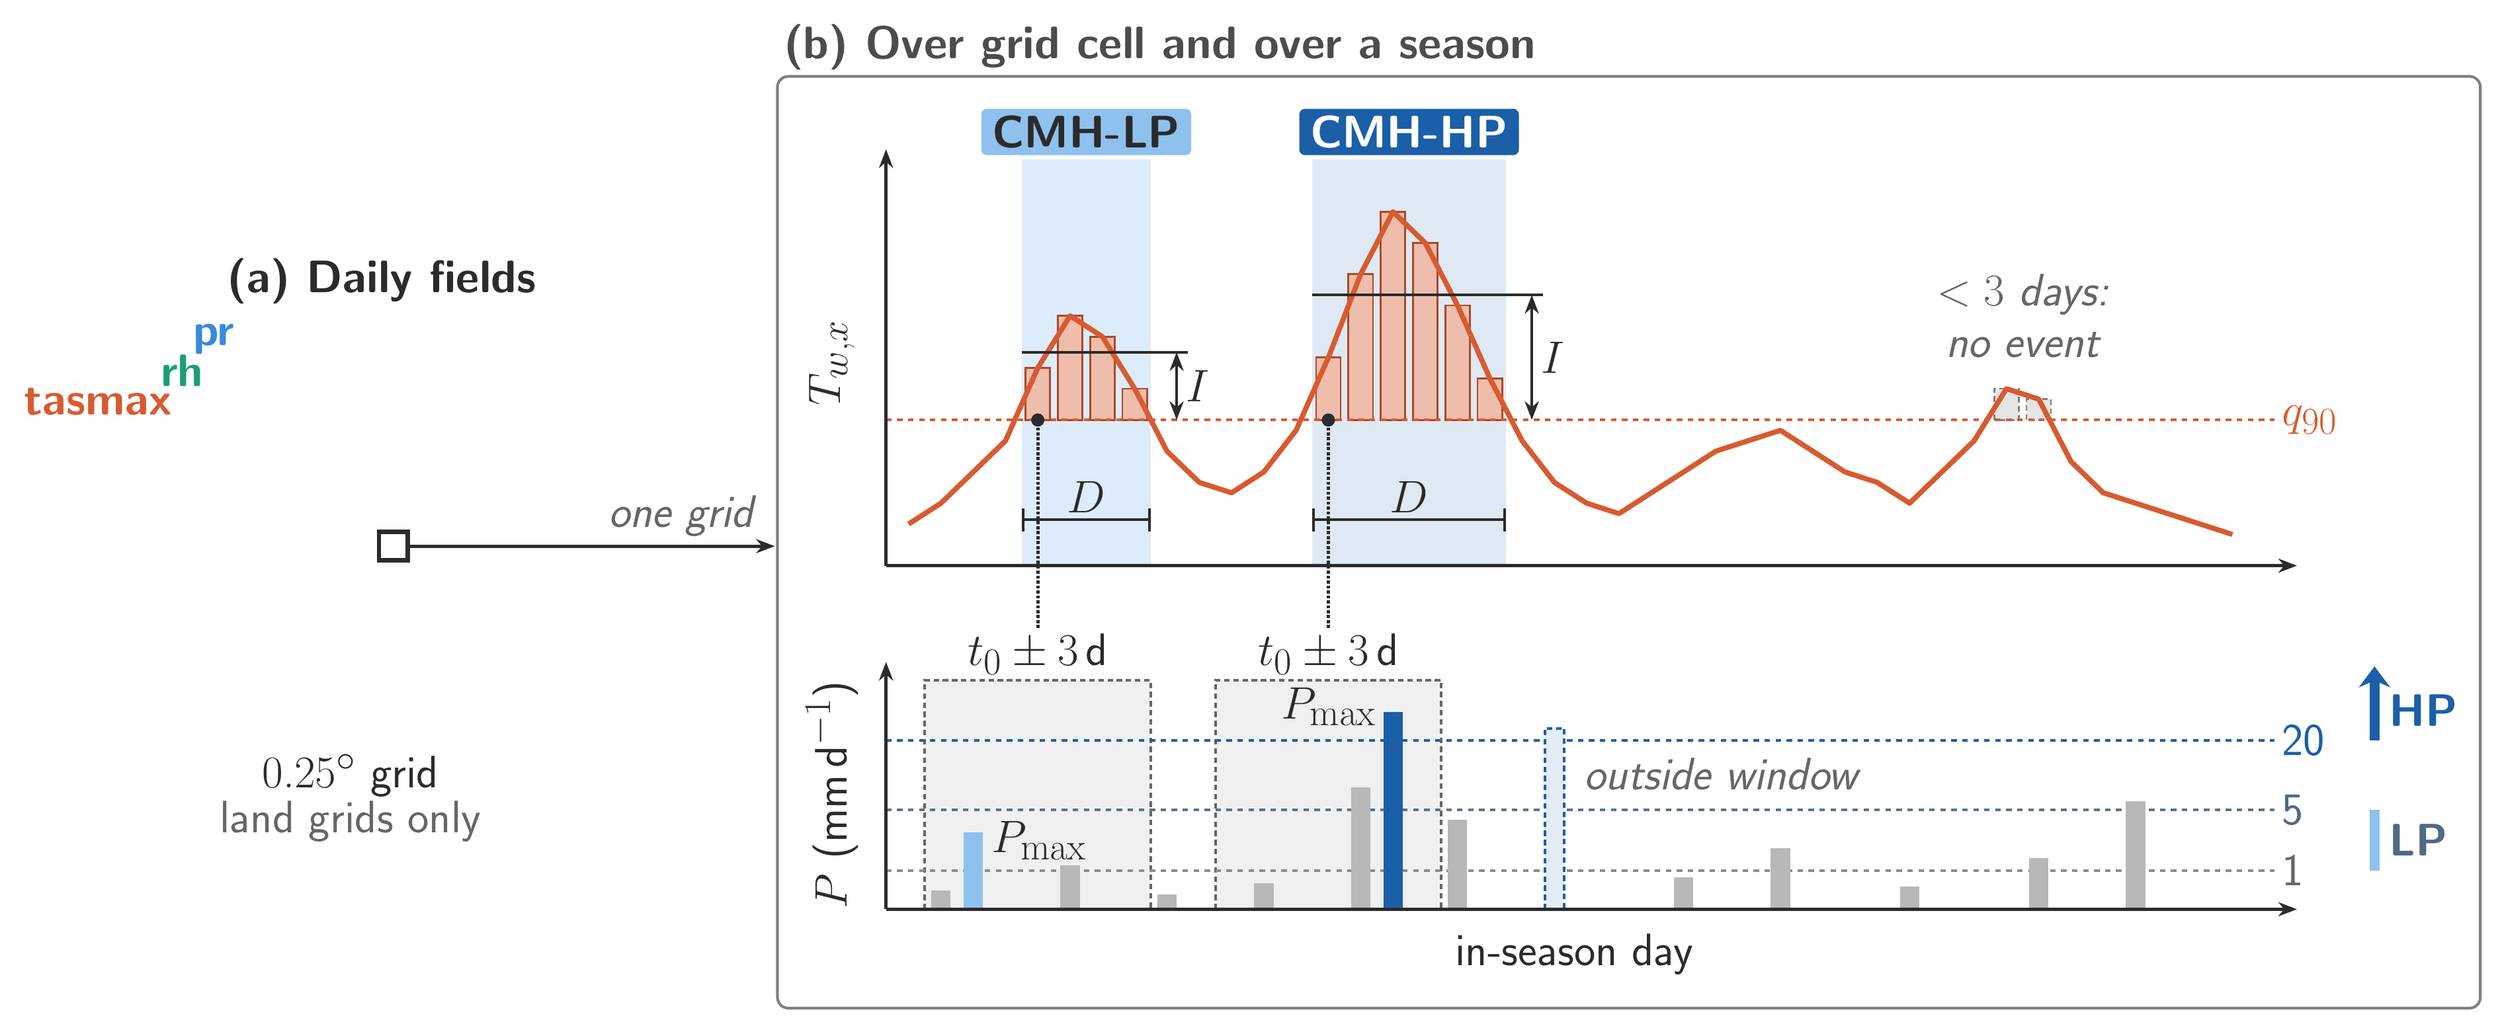
\begin{tikzpicture}[font=\Huge\sffamily, text=cInk, >={Stealth[length=3.6mm]},
  flow/.style={->, line width=1.9pt, cInk},
  ax/.style={->, line width=1.7pt, cInk},
  thr/.style={dashed, line width=1.5pt},
  lbl/.style={align=center, font=\Huge\sffamily, anchor=north},
  dim/.style={align=center, font=\Huge\sffamily, text=black!60, anchor=north},
  note/.style={align=center, font=\Huge\itshape, text=black!60},
  tag/.style={font=\Huge\bfseries, rounded corners=3pt, inner xsep=6pt, inner ysep=4pt, anchor=south},
  span/.style={{Bar[width=4.5mm]}-{Bar[width=4.5mm]}, line width=1.5pt, cInk}]

% ============================================================
%  (a) DAILY FIELDS ON THE 0.25-DEGREE GRID
% ============================================================
\def\L{6.6}
\hmap{3.90}{4.60}{\L}{12}{cV}{120}{9}
\hmap{3.30}{4.00}{\L}{12}{cH}{60}{9}
\hmap{2.70}{3.40}{\L}{12}{cT}{0}{9}
\node[font=\Huge\bfseries, text=cT, anchor=east] at (2.70,9.75) {tasmax};
\node[font=\Huge\bfseries, text=cH, anchor=east] at (3.30,10.35) {rh};
\node[font=\Huge\bfseries, text=cV, anchor=east] at (3.90,10.95) {pr};
\node[font=\Huge\bfseries, anchor=south] at (6.6,11.5) {(a) Daily fields};
\node[lbl] at (6.0,3.1) {$0.25^\circ$ grid};
\node[dim] at (6.0,2.2) {land grids only};
% selected grid grid and link to panel (b)
\draw[cInk, line width=2.4pt, fill=white, fill opacity=0.35] (6.55,6.70) rectangle ++(0.55,0.55);
\draw[flow] (7.10,6.975) -- (14.15,6.975);
\node[note, anchor=south] at (12.35,7.05) {one grid};

% ============================================================
%  (b) ONE GRID grid, ONE WARM SEASON
% ============================================================
\draw[black!50, line width=1.5pt, rounded corners=6pt] (14.2,-1.9) rectangle (46.9,16.0);
\node[anchor=south west, font=\Huge\bfseries, text=black!70] at (14.2,16.0) {(b) Over grid cell and over a season};
\node[rotate=90] at (15.25,10.5) {$T_{w,x}$};
\node[rotate=90] at (15.25,2.2) {$P$ (mm\,d$^{-1}$)};

% ---------- top: daily maximum wet-bulb temperature ----------
\begin{scope}[shift={(16.1,4.6)}, x=0.62cm, y=4.0cm]
% event columns and class tags
\fill[lightR!30] (4.5,0.5) rectangle (8.5,2.45);
\fill[heavyR!14] (13.5,0.5) rectangle (19.5,2.45);
\node[tag, fill=lightR] at (6.5,2.47) {CMH-LP};
\node[tag, fill=heavyR, text=white] at (16.5,2.47) {CMH-HP};
% event days (above q90 for >= 3 consecutive days)
\foreach \d/\v in {5/1.45,6/1.70,7/1.60,8/1.35,14/1.50,15/1.90,16/2.20,17/2.05,18/1.75,19/1.40}{
  \fill[cT!40, draw=cT!80!black, line width=1pt] (\d-0.38,1.2) rectangle (\d+0.38,\v);}
% exceedance shorter than 3 days: not an event
\foreach \d/\v in {35/1.35,36/1.30}{\fill[black!10, draw=black!50, densely dashed, line width=1pt] (\d-0.38,1.2) rectangle (\d+0.38,\v);}
% q90 threshold and T_w,x series
\draw[cT, thr] (0.3,1.2) -- (43.3,1.2) node[right, text=cT] {$q_{90}$};
\draw[cT, line width=2.8pt, line join=round] plot coordinates {
  (1,0.70) (2,0.80) (3,0.95) (4,1.10) (5,1.45) (6,1.70) (7,1.60) (8,1.35) (9,1.05) (10,0.90)
  (11,0.85) (12,0.95) (13,1.15) (14,1.50) (15,1.90) (16,2.20) (17,2.05) (18,1.75) (19,1.40) (20,1.10)
  (21,0.90) (22,0.80) (23,0.75) (24,0.85) (25,0.95) (26,1.05) (27,1.10) (28,1.15) (29,1.05) (30,0.95)
  (31,0.90) (32,0.80) (33,0.95) (34,1.10) (35,1.35) (36,1.30) (37,1.00) (38,0.85) (39,0.80) (40,0.75)
  (41,0.70) (42,0.65)};
% intensity I = mean exceedance above q90 over the event days
\foreach \a/\b/\m in {4.5/9.3/1.525,13.5/20.3/1.80}{
  \draw[cInk, line width=1.5pt] (\a,\m) -- (\b+0.35,\m);
  \draw[cInk, <->, line width=1.5pt] (\b,1.2) -- (\b,\m) node[midway, right=1pt] {$I$};}
% duration D of each event
\foreach \a/\b in {4.5/8.5,13.5/19.5}{\draw[span] (\a,0.72) -- (\b,0.72) node[midway, above=0pt] {$D$};}
\node[note] at (35.5,1.70) {$<3$ days:\\[-2pt]no event};
\draw[ax] (0.3,0.5) -- (44.0,0.5);
\draw[ax] (0.3,0.5) -- (0.3,2.5);
\end{scope}

% ---------- bottom: daily precipitation (log(1+P) scale) ----------
\begin{scope}[shift={(16.1,0)}, x=0.62cm, y=4.4cm]
% classification window t0 +/- 3 d, linked to the onset day
\foreach \t in {5,14}{
  \fill[black!6] (\t-3.5,0) rectangle (\t+3.5,1.0);
  \draw[black!60, densely dashed, line width=1.4pt] (\t-3.5,0) rectangle (\t+3.5,1.0);
  \node[anchor=south, inner sep=3pt] (w\t) at (\t,1.0) {$t_0\pm3$\,d};
  \draw[cInk, densely dotted, line width=1.7pt] (w\t.north) -- (\t,2.136);
  \fill[cInk] (\t,2.136) circle[radius=3.6pt];}
% precipitation thresholds: 1, 5 and 20 mm/d
\draw[black!45, thr] (0.3,0.168) -- (43.3,0.168) node[right, text=black!60] {1};
\draw[lightR!60!black, thr] (0.3,0.434) -- (43.3,0.434) node[right, text=lightR!55!black] {5};
\draw[heavyR, thr] (0.3,0.738) -- (43.3,0.738) node[right, text=heavyR] {20};
% P_max ranges defining each class
\draw[lightR, line width=5.5pt] (46.4,0.168) -- (46.4,0.434) node[midway, right=2pt, text=lightR!55!black, font=\Huge\bfseries] {LP};
\draw[heavyR, line width=5.5pt, -{Stealth[length=4mm, width=6mm]}] (46.4,0.738) -- (46.4,1.06) node[pos=0.4, right=2pt, text=heavyR, font=\Huge\bfseries] {HP};
% daily precipitation; coloured bars are P_max inside each window
\foreach \d/\h in {2/0.082,6/0.191,9/0.064,12/0.114,15/0.533,18/0.390,25/0.140,28/0.266,32/0.098,36/0.222,39/0.472}{\fill[black!28] (\d-0.3,0) rectangle (\d+0.3,\h);}
\fill[lightR] (2.7,0) rectangle (3.3,0.336);
\fill[heavyR] (15.7,0) rectangle (16.3,0.862);
% heavy precipitation outside the window
\fill[heavyR!12, draw=heavyR, densely dashed, line width=1.4pt] (20.7,0) rectangle (21.3,0.790);
\node[anchor=west, inner sep=2pt] at (3.45,0.30) {$P_{\max}$};
\node[anchor=east, inner sep=2pt] at (15.6,0.885) {$P_{\max}$};
\node[note, anchor=west, fill=white, inner sep=2pt] at (21.8,0.59) {outside window};
\draw[ax] (0.3,0) -- (44.0,0);
\draw[ax] (0.3,0) -- (0.3,1.08);
\end{scope}
\node[lbl] at (29.5,-0.35) {in-season day};
\end{tikzpicture}
\end{document}